\chapter{Evaluation}
\label{chap:evaluation}

This chapter evaluates the project as a whole with a focus on the development process, and whether the project meets the requirements set out in \autorefp{chap:requirements}. The chapter will also discuss the limitations of the project and potential future work.

\section{Project Timeline and Management}
\label{evaluation:timeline-management}

During the early stages of the academic year, starting a project was exciting and was progressing well. The problem would prove challenging over time, yet rewarding when understanding the fundamentals which build route planning systems. Time-management was key to ensure the project progressed at a steady pace despite the pressing deadlines of other modules. It was key to set out a plan and determine theoretical deadlines for development and writing of the report. Due to the rigorous time management and planning, the project swiftly began to move ahead of schedule, resulting in the initial Gantt chart  being revised to adjust for the rapid progress.

\begin{figure}[h!]
    \centering
    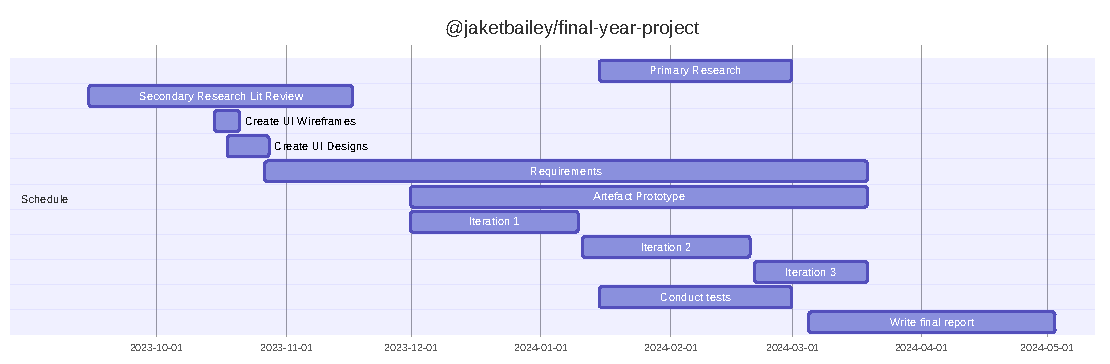
\includegraphics[width=1\linewidth]{figures/Old FYP Gantt - Timeline 1.pdf}
    \caption{Initial Gantt Chart}
    \label{fig:initial-gantt}
\end{figure}

\begin{figure}[h!]
    \centering
    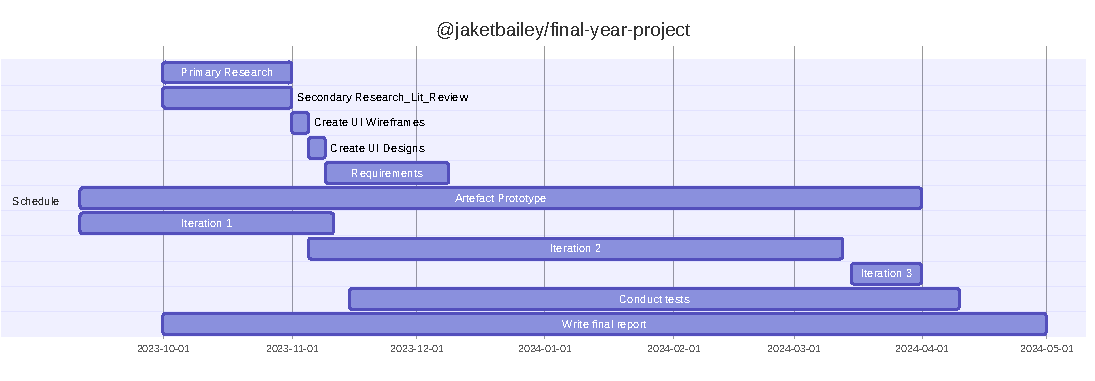
\includegraphics[width=1\linewidth]{figures/Actual FYP Gantt.pdf}
    \caption{Final Gantt Chart}
    \label{fig:final-gantt}
\end{figure}


\section{Evaluating Requirements}
\label{evaluation:requirements}

\begingroup
\setlength{\tabcolsep}{10pt} % Default value: 6pt
\renewcommand{\arraystretch}{1.5} % Default value: 1
\begin{table}[!htb]
\caption{Requirements Evaluation}
\label{evaluatedrq}
\small
    \begin{tabularx}{\textwidth}{ p{1cm} p{11cm} p{1cm} }
        \hline
        ID & Description & Met? \\ 
        \hline
        & \textbf{\hyperref[tab:user-story-01]{User Story 01}} \\
        \hyperref[SR:1]{SR1} & The system must provide a route configuration panel. & Y\\
        \hyperref[SR:2]{SR2} & The route configuration page must provide a starting and destination location input field. & Y\\
        \hyperref[SR:3]{SR3} & The route configuration page should suggest accurate geolocations based on the location inputs.  & Y\\
        \hyperref[SR:4]{SR4} & The route configuration page must determine the geolocation based on the user input. & Y\\
        \hyperref[SR:5]{SR5} & The route configuration page must plan the route once two or more locations are input. & Y\\
        \hline
        & \textbf{\hyperref[tab:user-story-02]{User Story 02}}  \\
        \hyperref[SR:6]{SR6} & The system must provide an overlay window to allow the user to update routing preferences. & Y\\
        \hyperref[SR:7]{SR7} & The update preferences overlay must provide options to 'avoid' along the route. & Y\\
        \hyperref[SR:8]{SR8} & The update preferences overlay must provide a 'via' user input field. & Y\\ 
        \hyperref[SR:9]{SR9} & The update preferences overlay must provide a 'leave time' user input field. & Y\\ 
        \hyperref[SR:10]{SR10} & The update preferences overlay must provide a 'arrive time' user input field. & Y\\ 
        \hyperref[SR:11]{SR11} & The update preferences overlay must provide a 'round trip' user input field. & Y\\ 
        \hline
        & \textbf{\hyperref[tab:user-story-03]{User Story 03}}  \\
        \hyperref[SR:12]{SR12} & The system must provide an option to export the planned route. & Y \\
        \hyperref[SR:13]{SR13} & The system must provide an export feature to export the route to the 'GPX' file format. & Y\\
        \hyperref[SR:14]{SR14} & The system must provide an export feature to export the route to the 'GeoJSON' file format. & Y\\ 
        \hyperref[SR:15]{SR15} & The system must provide an export online (to Google Drive, OneDrive and/or other cloud services) & Y\\
        \hline
        & \textbf{\hyperref[tab:user-story-04]{User Story 04}}  \\
        \hyperref[SR:16]{SR16} & The system must provide a share functionality overlay. & Y \\
        \hyperref[SR:17]{SR17} & The share overlay must provide an option to share direct over email. & Y\\
        \hyperref[SR:18]{SR18} & The system must provide an option to share the route direct to Strava. & Y\\ 
        \hline
    \end{tabularx}
\end{table}
\clearpage

\begin{table}[!htb]
    \ContinuedFloat
    \caption{Requirements Evaluation Continued}
    \label{evaluatedrqextended}
    \small
    \begin{tabularx}{\textwidth}{ p{1cm} p{11cm} p{1cm} }
        \hline
        SR & Description & Met? \\ 
        \hline
        & \textbf{\hyperref[tab:user-story-05]{User Story 05}} \\
        \hyperref[SR:19]{SR19} & The system must provide the user with a weather condition overlay. & Y \\
        \hyperref[SR:20]{SR20} & The weather condition overlay must provide the user with the weather for the current day. & Y\\
        \hyperref[SR:21]{SR21} & The weather condition overlay must provide the user with the weather for the next week. & Y\\
        \hyperref[SR:22]{SR22} & The weather condition overlay must provide the user with the option to enable weather conditions in the route planning algorithm. & N\\ 
        \hyperref[SR:23]{SR23} & The weather condition overlay must provide the user with suggestions on the best days to cycle. & N\\
        \hyperref[SR:24]{SR24} & An option to include weather in route planning should be provided, ensuring the user enters the planned day to ride & N\\ 
        \hline
        & \textbf{\hyperref[tab:user-story-06]{User Story 06}}  \\
        \hyperref[SR:25]{SR25} & The system must provide the user with an interactive map to display the planned route. & Y \\
        \hyperref[SR:26]{SR26} & The interactive map must allow the user to zoom into parts of the planned route. & Y\\
        \hyperref[SR:27]{SR27} & The interactive map must allow the user to select parts of the route and receive detailed information about that subsection of the route. & Y\\
        \hyperref[SR:28]{SR28} & The interactive map must allow the user to select and drag the planned route to modify its path. & Y\\ 
        \hyperref[SR:29]{SR29} & The system must display an elevation graph for the planned route beneath the interactive map. & Y\\
        \hyperref[SR:30]{SR30} & The system must allow the user to measure chosen sections of the route & Y\\
        \hyperref[SR:31]{SR31} & The system must provide multiple map layers to give users the greater options when viewing the route & Y\\ 
        \hline
        & \textbf{\hyperref[tab:user-story-07]{User Story 07}}  \\
        \hyperref[SR:32]{SR32} & The system must provide a user input modal to input Hazard and Infrastructure Data. & Y \\
        \hyperref[SR:33]{SR33} & The hazard input modal must provide a Type drop-down menu based on the OSM Hazard Types. & Y\\
        \hyperref[SR:34]{SR34} & The hazard input modal must provide a date entry point to specify the date the hazard was seen. & Y\\
        \hyperref[SR:35]{SR35} & The hazard input modal must provide a submit button to add the hazard to the hazard index. & Y\\
        \hyperref[SR:36]{SR36} & The infrastructure input modal must provide a Type drop-down menu with different types of cycling/road infrastructure & Y\\
        \hyperref[SR:37]{SR37} & The infrastructure input modal must provide a date entry point to specify when the bad infrastructure was found & Y\\
        \hline
    \end{tabularx}
\end{table}
\clearpage

\begin{table}[!htb]
    \ContinuedFloat
    \caption{Requirements Evaluation Continued}
    \label{evaluatedrqextended2}
    \small
    \begin{tabularx}{\textwidth}{ p{1cm} p{11cm} p{1cm} }
        \hline
        SR & Description & Met? \\ 
        \hline
        & \textbf{\hyperref[tab:user-story-07]{User Story 07 Cont.}}  \\
        \hyperref[SR:38]{SR38} & The infrastructure input modal must provide an input box providing the user with the option to supply more detail & Y\\
        \hyperref[SR:39]{SR39} & Both Hazard and Infrastructure data should be displayed on the map, with an option to toggle on/off, and report errors & Y\\
        \hline
        & \textbf{\hyperref[tab:user-story-08]{User Story 08}}  \\
        \hyperref[SR:40]{SR40} & The system must provide a map layer to include key waypoints. & Y \\
        \hyperref[SR:41]{SR41} & The waypoint layer must provide locations of accommodation along the route. & Y\\
        \hyperref[SR:42]{SR42} & The waypoint layer must provide locations of tourist points along the route & Y\\
        \hyperref[SR:43]{SR43} & The waypoint layers must be able to be toggled on and off & Y\\
        \hyperref[SR:44]{SR44} & Each waypoint must be clickable to provide extra detail on each point & Y\\
        \hyperref[SR:45]{SR45} & Each waypoint must have a button to add stop along the route and the route will be re-plotted via the waypoint. & Y\\
        \hline
        & \textbf{\hyperref[tab:user-story-09]{User Story 09}}  \\
        \hyperref[SR:46]{SR46} & The system must provide an option within the route planning modal to select the rider type. & Y\\
        \hyperref[SR:47]{SR47} & The system must provide an option within the route planning modal to select the fitness level of the rider. & N\\
        \hline
        & \textbf{\hyperref[tab:user-story-10]{User Story 10}}  \\
        \hyperref[SR:48]{SR48} & The system must provide an import option for GPX files. & Y\\
        \hyperref[SR:49]{SR49} & The system must provide an import option for GeoJSON files. & Y\\
        \hline
        & \textbf{\hyperref[tab:user-story-11]{User Story 11}} \\
        \hyperref[SR:50]{SR50} & The system must provide an export to Garmin Routes. & Y\\
        \hyperref[SR:51]{SR51} & The system must provide an option to share to different social media platforms. & Y\\
        \hline
    \end{tabularx}
\end{table}
\endgroup

\section{Limitations}
\label{evaluation:limitations}

\section{Future Work}
\label{evaluation:future}

